
%-----------------------------------------------------------------------------
% PACKAGES AND OTHER DOCUMENT CONFIGURATIONS
%-----------------------------------------------------------------------------

\documentclass[11pt,addpoints,answers]{exam}
\usepackage[margin=1in]{geometry}
\usepackage{amsmath, amsfonts}
\usepackage{enumerate}
\usepackage{graphicx}
\usepackage{titling}
\usepackage{url}
\usepackage{xfrac}
\usepackage{natbib}
\usepackage{amssymb}
\usepackage{amsthm}
\usepackage{paralist}
\usepackage{epstopdf}
\usepackage{tabularx}
\usepackage{longtable}
\usepackage{multirow}
\usepackage{multicol}
\usepackage[colorlinks=true,urlcolor=blue]{hyperref}
\usepackage{algorithm}
\usepackage{algorithmicx}
\usepackage[noend]{algpseudocode}
\usepackage{float}
\usepackage{enumerate}
\usepackage{array}
\usepackage{environ}
\usepackage{times}
\usepackage{textcomp}
\usepackage{caption}
\usepackage{parskip} % For NIPS style paragraphs.
\usepackage[compact]{titlesec} % Less whitespace around titles
\usepackage[inline]{enumitem} % For inline enumerate* and itemize*
\usepackage{datetime}
\usepackage{comment}
% \usepackage{minted}
\usepackage{lastpage}
\usepackage{color}
\usepackage{xcolor}
\usepackage[final]{listings}
\usepackage{tikz}
\usetikzlibrary{shapes,decorations}
\usepackage{framed}
\usepackage{booktabs}
\usepackage{cprotect}
\usepackage{verbatimbox}
\usepackage{multicol}
\usepackage{hyperref}
\usepackage{subcaption}
\usepackage{mathtools} % For drcases
\usepackage{cancel}
\usepackage[many]{tcolorbox}
\usepackage{soul}
\usepackage[bottom]{footmisc}
\usepackage{bm}
\usepackage{wasysym}

\usepackage{tikz}
\usetikzlibrary{shapes.geometric}
\usetikzlibrary{positioning, arrows, automata}

\newtcolorbox[]{your_solution}[1][]{%
    % breakable,
    enhanced,
    nobeforeafter,
    colback=white,
    title=Your Answer,
    sidebyside align=top,
    box align=top,
    #1
}

%%%%%%%%%%%%%%%%%%%%%%%%%%%%%%%%%%%%%%%%%%%
% Rotated Column Headers                  %
%%%%%%%%%%%%%%%%%%%%%%%%%%%%%%%%%%%%%%%%%%%
\usepackage{adjustbox}
\usepackage{array}

%https://tex.stackexchange.com/questions/32683/rotated-column-titles-in-tabular

\newcolumntype{R}[2]{%
    >{\adjustbox{angle=#1,lap=\width-(#2)}\bgroup}%
    l%
    <{\egroup}%
}
\newcommand*\rot{\multicolumn{1}{R{45}{1em}}}% no optional argument here, please!


%%%%%%%%%%%%%%%%%%%%%%%%%%%%%%%%%%%%%%%%%%%
% Better numbering                        %
%%%%%%%%%%%%%%%%%%%%%%%%%%%%%%%%%%%%%%%%%%%

% \numberwithin{equation}{section} % Number equations within sections (i.e. 1.1, 1.2, 2.1, 2.2 instead of 1, 2, 3, 4)
% \numberwithin{figure}{section} % Number figures within sections (i.e. 1.1, 1.2, 2.1, 2.2 instead of 1, 2, 3, 4)
% \numberwithin{table}{section} % Number tables within sections (i.e. 1.1, 1.2, 2.1, 2.2 instead of 1, 2, 3, 4)

%%%%%%%%%%%%%%%%%%%%%%%%%%%%%%%%%%%%%%%%%%
% Custom commands                        %
%%%%%%%%%%%%%%%%%%%%%%%%%%%%%%%%%%%%%%%%%%

\newcommand{\vc}[1]{\boldsymbol{#1}}
\newcommand{\adj}[1]{\frac{d J}{d #1}}
\newcommand{\chain}[2]{\adj{#2} = \adj{#1}\frac{d #1}{d #2}}

\newcommand{\independent}{\perp\!\!\!\perp  }

\newcommand{\R}{\mathbb{R}}
\newcommand{\blackcircle}{\tikz\draw[black,fill=black] (0,0) circle (1ex);}
\renewcommand{\circle}{\tikz\draw[black] (0,0) circle (1ex);}

\newcommand{\emptysquare}{{\LARGE $\square$}\ \ }
\newcommand{\filledsquare}{{\LARGE $\boxtimes$}\ \ }
\newcommand{\emptycircle}{{\LARGE $\fullmoon$}\ \ }
\newcommand{\filledcircle}{{\LARGE $\newmoon$}\ \ }


% mathcal
\newcommand{\Ac}{\mathcal{A}}
\newcommand{\Bc}{\mathcal{B}}
\newcommand{\Cc}{\mathcal{C}}
\newcommand{\Dc}{\mathcal{D}}
\newcommand{\Ec}{\mathcal{E}}
\newcommand{\Fc}{\mathcal{F}}
\newcommand{\Gc}{\mathcal{G}}
\newcommand{\Hc}{\mathcal{H}}
\newcommand{\Ic}{\mathcal{I}}
\newcommand{\Jc}{\mathcal{J}}
\newcommand{\Kc}{\mathcal{K}}
\newcommand{\Lc}{\mathcal{L}}
\newcommand{\Mc}{\mathcal{M}}
\newcommand{\Nc}{\mathcal{N}}
\newcommand{\Oc}{\mathcal{O}}
\newcommand{\Pc}{\mathcal{P}}
\newcommand{\Qc}{\mathcal{Q}}
\newcommand{\Rc}{\mathcal{R}}
\newcommand{\Sc}{\mathcal{S}}
\newcommand{\Tc}{\mathcal{T}}
\newcommand{\Uc}{\mathcal{U}}
\newcommand{\Vc}{\mathcal{V}}
\newcommand{\Wc}{\mathcal{W}}
\newcommand{\Xc}{\mathcal{X}}
\newcommand{\Yc}{\mathcal{Y}}
\newcommand{\Zc}{\mathcal{Z}}

% mathbb
\newcommand{\Ab}{\mathbb{A}}
\newcommand{\Bb}{\mathbb{B}}
\newcommand{\Cb}{\mathbb{C}}
\newcommand{\Db}{\mathbb{D}}
\newcommand{\Eb}{\mathbb{E}}
\newcommand{\Fb}{\mathbb{F}}
\newcommand{\Gb}{\mathbb{G}}
\newcommand{\Hb}{\mathbb{H}}
\newcommand{\Ib}{\mathbb{I}}
\newcommand{\Jb}{\mathbb{J}}
\newcommand{\Kb}{\mathbb{K}}
\newcommand{\Lb}{\mathbb{L}}
\newcommand{\Mb}{\mathbb{M}}
\newcommand{\Nb}{\mathbb{N}}
\newcommand{\Ob}{\mathbb{O}}
\newcommand{\Pb}{\mathbb{P}}
\newcommand{\Qb}{\mathbb{Q}}
\newcommand{\Rb}{\mathbb{R}}
\newcommand{\Sb}{\mathbb{S}}
\newcommand{\Tb}{\mathbb{T}}
\newcommand{\Ub}{\mathbb{U}}
\newcommand{\Vb}{\mathbb{V}}
\newcommand{\Wb}{\mathbb{W}}
\newcommand{\Xb}{\mathbb{X}}
\newcommand{\Yb}{\mathbb{Y}}
\newcommand{\Zb}{\mathbb{Z}}

% mathbf lowercase
\newcommand{\av}{\mathbf{a}}
\newcommand{\bv}{\mathbf{b}}
\newcommand{\cv}{\mathbf{c}}
\newcommand{\dv}{\mathbf{d}}
\newcommand{\ev}{\mathbf{e}}
\newcommand{\fv}{\mathbf{f}}
\newcommand{\gv}{\mathbf{g}}
\newcommand{\hv}{\mathbf{h}}
\newcommand{\iv}{\mathbf{i}}
\newcommand{\jv}{\mathbf{j}}
\newcommand{\kv}{\mathbf{k}}
\newcommand{\lv}{\mathbf{l}}
\newcommand{\mv}{\mathbf{m}}
\newcommand{\nv}{\mathbf{n}}
\newcommand{\ov}{\mathbf{o}}
\newcommand{\pv}{\mathbf{p}}
\newcommand{\qv}{\mathbf{q}}
\newcommand{\rv}{\mathbf{r}}
\newcommand{\sv}{\mathbf{s}}
\newcommand{\tv}{\mathbf{t}}
\newcommand{\uv}{\mathbf{u}}
\newcommand{\vv}{\mathbf{v}}
\newcommand{\wv}{\mathbf{w}}
\newcommand{\xv}{\mathbf{x}}
\newcommand{\yv}{\mathbf{y}}
\newcommand{\zv}{\mathbf{z}}

% mathbf uppercase
\newcommand{\Av}{\mathbf{A}}
\newcommand{\Bv}{\mathbf{B}}
\newcommand{\Cv}{\mathbf{C}}
\newcommand{\Dv}{\mathbf{D}}
\newcommand{\Ev}{\mathbf{E}}
\newcommand{\Fv}{\mathbf{F}}
\newcommand{\Gv}{\mathbf{G}}
\newcommand{\Hv}{\mathbf{H}}
\newcommand{\Iv}{\mathbf{I}}
\newcommand{\Jv}{\mathbf{J}}
\newcommand{\Kv}{\mathbf{K}}
\newcommand{\Lv}{\mathbf{L}}
\newcommand{\Mv}{\mathbf{M}}
\newcommand{\Nv}{\mathbf{N}}
\newcommand{\Ov}{\mathbf{O}}
\newcommand{\Pv}{\mathbf{P}}
\newcommand{\Qv}{\mathbf{Q}}
\newcommand{\Rv}{\mathbf{R}}
\newcommand{\Sv}{\mathbf{S}}
\newcommand{\Tv}{\mathbf{T}}
\newcommand{\Uv}{\mathbf{U}}
\newcommand{\Vv}{\mathbf{V}}
\newcommand{\Wv}{\mathbf{W}}
\newcommand{\Xv}{\mathbf{X}}
\newcommand{\Yv}{\mathbf{Y}}
\newcommand{\Zv}{\mathbf{Z}}

% bold greek lowercase
\newcommand{\alphav     }{\boldsymbol \alpha     }
\newcommand{\betav      }{\boldsymbol \beta      }
\newcommand{\gammav     }{\boldsymbol \gamma     }
\newcommand{\deltav     }{\boldsymbol \delta     }
\newcommand{\epsilonv   }{\boldsymbol \epsilon   }
\newcommand{\varepsilonv}{\boldsymbol \varepsilon}
\newcommand{\zetav      }{\boldsymbol \zeta      }
\newcommand{\etav       }{\boldsymbol \eta       }
\newcommand{\thetav     }{\boldsymbol \theta     }
\newcommand{\varthetav  }{\boldsymbol \vartheta  }
\newcommand{\iotav      }{\boldsymbol \iota      }
\newcommand{\kappav     }{\boldsymbol \kappa     }
\newcommand{\varkappav  }{\boldsymbol \varkappa  }
\newcommand{\lambdav    }{\boldsymbol \lambda    }
\newcommand{\muv        }{\boldsymbol \mu        }
\newcommand{\nuv        }{\boldsymbol \nu        }
\newcommand{\xiv        }{\boldsymbol \xi        }
\newcommand{\omicronv   }{\boldsymbol \omicron   }
\newcommand{\piv        }{\boldsymbol \pi        }
\newcommand{\varpiv     }{\boldsymbol \varpi     }
\newcommand{\rhov       }{\boldsymbol \rho       }
\newcommand{\varrhov    }{\boldsymbol \varrho    }
\newcommand{\sigmav     }{\boldsymbol \sigma     }
\newcommand{\varsigmav  }{\boldsymbol \varsigma  }
\newcommand{\tauv       }{\boldsymbol \tau       }
\newcommand{\upsilonv   }{\boldsymbol \upsilon   }
\newcommand{\phiv       }{\boldsymbol \phi       }
\newcommand{\varphiv    }{\boldsymbol \varphi    }
\newcommand{\chiv       }{\boldsymbol \chi       }
\newcommand{\psiv       }{\boldsymbol \psi       }
\newcommand{\omegav     }{\boldsymbol \omega     }

% bold greek uppercase
\newcommand{\Gammav     }{\boldsymbol \Gamma     }
\newcommand{\Deltav     }{\boldsymbol \Delta     }
\newcommand{\Thetav     }{\boldsymbol \Theta     }
\newcommand{\Lambdav    }{\boldsymbol \Lambda    }
\newcommand{\Xiv        }{\boldsymbol \Xi        }
\newcommand{\Piv        }{\boldsymbol \Pi        }
\newcommand{\Sigmav     }{\boldsymbol \Sigma     }
\newcommand{\Upsilonv   }{\boldsymbol \Upsilon   }
\newcommand{\Phiv       }{\boldsymbol \Phi       }
\newcommand{\Psiv       }{\boldsymbol \Psi       }
\newcommand{\Omegav     }{\boldsymbol \Omega     }

%%%%%%%%%%%%%%%%%%%%%%%%%%%%%%%%%%%%%%%%%%%
% Code highlighting with listings         %
%%%%%%%%%%%%%%%%%%%%%%%%%%%%%%%%%%%%%%%%%%%

\definecolor{bluekeywords}{rgb}{0.13,0.13,1}
\definecolor{greencomments}{rgb}{0,0.5,0}
\definecolor{redstrings}{rgb}{0.9,0,0}
\definecolor{light-gray}{gray}{0.95}

\newcommand{\MYhref}[3][blue]{\href{#2}{\color{#1}{#3}}}%

\definecolor{dkgreen}{rgb}{0,0.6,0}
\definecolor{gray}{rgb}{0.5,0.5,0.5}
\definecolor{mauve}{rgb}{0.58,0,0.82}

\lstdefinelanguage{Shell}{
  keywords={tar, cd, make},
  %keywordstyle=\color{bluekeywords}\bfseries,
  alsoletter={+},
  ndkeywords={python, py, javac, java, gcc, c, g++, cpp, .txt, octave, m, .tar},
  %ndkeywordstyle=\color{bluekeywords}\bfseries,
  identifierstyle=\color{black},
  sensitive=false,
  comment=[l]{//},
  morecomment=[s]{/*}{*/},
  commentstyle=\color{purple}\ttfamily,
  %stringstyle=\color{red}\ttfamily,
  morestring=[b]',
  morestring=[b]",
  backgroundcolor = \color{light-gray}
}

\lstset{columns=fixed, basicstyle=\ttfamily,
    backgroundcolor=\color{light-gray},xleftmargin=0.5cm,frame=tlbr,framesep=4pt,framerule=0pt}


%%%%%%%%%%%%%%%%%%%%%%%%%%%%%%%%%%%%%%%%%%%
% Custom box for highlights               %
%%%%%%%%%%%%%%%%%%%%%%%%%%%%%%%%%%%%%%%%%%%

% Define box and box title style
\tikzstyle{mybox} = [fill=blue!10, very thick,
    rectangle, rounded corners, inner sep=1em, inner ysep=1em]

% \newcommand{\notebox}[1]{
% \begin{tikzpicture}
% \node [mybox] (box){%
%     \begin{minipage}{\textwidth}
%     #1
%     \end{minipage}
% };
% \end{tikzpicture}%
% }

\NewEnviron{notebox}{

\begin{tikzpicture}
\node [mybox] (box){
    \begin{minipage}{\textwidth}
        \BODY
    \end{minipage}
};
\end{tikzpicture}
}

%%%%%%%%%%%%%%%%%%%%%%%%%%%%%%%%%%%%%%%%%%%
% Commands showing / hiding solutions     %
%%%%%%%%%%%%%%%%%%%%%%%%%%%%%%%%%%%%%%%%%%%

%% To HIDE SOLUTIONS (to post at the website for students), set this value to 0: 
% \def\issoln{0}
\def\issoln{0}
% Some commands to allow solutions to be embedded in the assignment file.
\ifcsname issoln\endcsname \else \def\issoln{1} \fi
% Default to an empty solutions environ.
\NewEnviron{soln}{}{}
\if\issoln 1
% Otherwise, include solutions as below.
\RenewEnviron{soln}{
    \leavevmode\color{red}\ignorespaces
    % \textbf{Solution} \BODY
    \BODY
}{}
\fi

%% To HIDE TAGS set this value to 0:
\def\showtags{1}
%%%%%%%%%%%%%%%%
\ifcsname showtags\endcsname \else \def\showtags{1} \fi
% Default to an empty tags environ.
\NewEnviron{tags}{}{}
\if\showtags 1
% Otherwise, include solutions as below.
\RenewEnviron{tags}{
    \fbox{
    \leavevmode\color{blue}\ignorespaces
    \textbf{TAGS:} \texttt{\url{\BODY}}
    }
    \vspace{-.5em}
}{}
\fi

%%%%%%%%%%%%%%%%%%%%%%%%%%%%%%%%%%%%%%%%%%%
% Commands for customizing the assignment %
%%%%%%%%%%%%%%%%%%%%%%%%%%%%%%%%%%%%%%%%%%%

\newcommand{\courseName}{10-301/10-601 Introduction to Machine Learning (Spring 2021)}
\newcommand{\hwName}{Homework 7: Graphical Models}
\newcommand{\dueDate}{Friday, April 30, 2021 11:59 PM}


\title{\textsc{\hwName}
%\thanks{Compiled on \today{} at \currenttime{}}
} % Title


\author{\courseName\\
\url{https://www.cs.cmu.edu/~10601/} \\
DUE: \dueDate{} \\ 
}

\date{}

%%%%%%%%%%%%%%%%%%%%%%%%%%%%%%%%%%%%%%%%%%%%%%%%%
% Useful commands for typesetting the questions %
%%%%%%%%%%%%%%%%%%%%%%%%%%%%%%%%%%%%%%%%%%%%%%%%%

\newcommand \expect {\mathbb{E}}
\newcommand \mle [1]{{\hat #1}^{\rm MLE}}
\newcommand \map [1]{{\hat #1}^{\rm MAP}}
\newcommand \argmax {\operatorname*{argmax}}
\newcommand \argmin {\operatorname*{argmin}}
\newcommand \code [1]{{\tt #1}}
\newcommand \datacount [1]{\#\{#1\}}
\newcommand \ind [1]{\mathbb{I}\{#1\}}

%%%%%%%%%%%%%%%%%%%%%%%%%%
% Document configuration %
%%%%%%%%%%%%%%%%%%%%%%%%%%

% Don't display a date in the title and remove the white space
\predate{}
\postdate{}
\date{}

% Don't display an author and remove the white space
%\preauthor{}
%\postauthor{}

%%%%%%%%%%%%%%%%%%
% Begin Document %
%%%%%%%%%%%%%%%%%% 

\begin{document}

\maketitle

\begin{notebox}
\paragraph{Summary} In this assignment you will go through exercises on MAP/MLE and learning graphical models with and without missing data. Finally, you will implement Gaussian Naive Bayes to predict a word category given the real-valued voxels of a human fMRI.
\end{notebox}\section*{START HERE: Instructions}
\begin{itemize}

\item \textbf{Collaboration Policy}: Please read the collaboration policy here: \url{https://www.cs.cmu.edu/~10601}

\item\textbf{Late Submission Policy:} See the late submission policy here: \url{https://www.cs.cmu.edu/~10601}

\item\textbf{Submitting your work:} You will use Gradescope to submit
  answers to all questions and code. Please
  follow instructions at the end of this PDF to correctly submit all your code to Gradescope.

  \begin{itemize}
    
 % COMMENT IF NOT USING CANVAS
\begin{comment}
  \item \textbf{Canvas:} Canvas (\url{https://canvas.cmu.edu}) will be
    used for quiz-style problems (e.g. multiple choice, true / false,
    numerical answers). Grading is done automatically.
    %
    You may only \textbf{submit once} on canvas, so be sure of your
    answers before you submit. However, canvas allows you to work on
    your answers and then close out of the page and it will save your
    progress.  You will not be granted additional submissions, so
    please be confident of your solutions when you are submitting your
    assignment.
    %
    {\color{red} The above is true for future assignments, but this one
    allows {\bf unlimited submissions}.}
\end{comment}
    
  % COMMENT IF NOT USING GRADESCOPE
   \item \textbf{Written:} For written problems such as short answer, multiple choice, derivations, proofs, or plots, please use the provided template. Submissions must be written in LaTeX.
   Each derivation/proof should be completed in the boxes provided. If you do not follow the template, your assignment may not be graded correctly by our AI assisted grader.

  %   COMMENT IF NOT USING GRADESCOPE AUTOGRADER
  \item \textbf{Programming:} You will submit your code for programming questions on the homework to Gradescope (\url{https://gradescope.com}). After uploading your code, our grading scripts will autograde your assignment by running your program on a virtual machine (VM). When you are developing, check that the version number of the programming language environment (e.g. Python 3.6.9, OpenJDK 11.0.5, g++ 7.4.0) and versions of permitted libraries (e.g.  \texttt{numpy} 1.17.0 and \texttt{scipy} 1.4.1) match those used on Gradescope. You have unlimited Gradescope programming submissions. However, we recommend debugging your implementation on your local machine (or the Linux servers) and making sure your code is running correctly first before submitting you code to Gradescope.

  \end{itemize}
  
\item\textbf{Materials:} The data that you will need in order to complete this assignment is posted along with the writeup and template on Piazza.

\end{itemize}


\begin{notebox}
\paragraph{Linear Algebra Libraries} When implementing machine learning algorithms, it is often convenient to have a linear algebra library at your disposal. In this assignment, Java users may use EJML\footnote{\url{https://ejml.org}} or ND4J\footnote{\url{https://deeplearning4j.org/docs/latest/nd4j-overview}} and C++ users Eigen\footnote{\url{http://eigen.tuxfamily.org/}}. Details below. 
%
(As usual, Python users have NumPy.)
%
\begin{description}
\item[EJML for Java] EJML is a pure Java linear algebra package with three interfaces. We strongly recommend using the SimpleMatrix interface. The autograder will use EJML version 0.38. When compiling and running your code, we will add the additional command line argument \small{\lstinline{-cp "linalg_lib/ejml-v0.38-libs/*:linalg_lib/nd4j-v1.0.0-beta7-libs/*:./"}}
to ensure that all the EJML jars are on the classpath as well as your code. 

\item[ND4J for Java] ND4J is a library for multidimensional tensors with an interface akin to Python's NumPy. The autograder will use ND4J version 1.0.0-beta7. When compiling and running your code, we will add the additional command line argument \small{\lstinline{-cp "linalg_lib/ejml-v0.38-libs/*:linalg_lib/nd4j-v1.0.0-beta7-libs/*:./"}} to ensure that all the ND4J jars are on the classpath as well as your code. 

\item[Eigen for C++] Eigen is a header-only library, so there is no linking to worry about---just \lstinline{#include} whatever components you need. The autograder will use Eigen version 3.3.7. The command line arguments above demonstrate how we will call you code. When compiling your code we will include, the argument \lstinline{-I./linalg_lib} in order to include the \lstinline{linalg_lib/Eigen} subdirectory, which contains all the headers.

\end{description} 
We have included the correct versions of EJML/ND4J/Eigen in the \lstinline{linalg_lib.zip} posted on the Piazza Resources page for your convenience. It contains the same \lstinline{linalg_lib/} directory that we will include in the current working directory when running your tests. Do {\bf not} include EJML, ND4J, or Eigen in your homework submission; the autograder will ensure that they are in place. 
\end{notebox}\clearpage

{\LARGE \bf Written Questions (60 points)}
\begin{questions}

\section{Short Questions}

\begin{table}[H] % need to change these numbers
    \centering
    \begin{tabular}{|c|c|c|c|}
    \hline
        $\mathbf{X_1}$ & $\mathbf{X_2}$ & $\mathbf{X_3}$ & Probability  \\  \hline
        $0$ & $0$ & $0$ & 0.15 \\  \hline
        $1$ & $0$  & $0$ & 0.05   \\  \hline
        $0$ & $1$  & $0$ & 0.15   \\  \hline
        $1$ & $1$  & $0$ & 0.05   \\  \hline
        $0$ & $0$  & $1$ & 0.1   \\  \hline
        $1$ & $0$  & $1$ & 0.3   \\  \hline
        $0$ & $1$  & $1$ & 0.05   \\  \hline
        $1$ & $1$  & $1$ & 0.15   \\  \hline
    \end{tabular}
    \caption{Joint Probability Table}
\end{table}

\begin{questions}

\question[2] What's the value of $P(X_1=1)$?

\begin{your_solution}[title=Your answer:,height=2cm,width=5cm]
\end{your_solution}

\question[2] What's the value of $P(X_1=0 | X_3=1)$?

\begin{your_solution}[title=Your answer:,height=2cm,width=5cm]
\end{your_solution}


\question[3] Is $(X_1 \independent X_2) | X_3$?  (i.e., is $X_1$ conditionally independent of $X_2$ given $X_3$?)

\textbf{Select one:}
    \begin{checkboxes}
        \choice True
        \choice False
\end{checkboxes}


\question[3] Is $X_1 \independent X_2 $?

\textbf{Select one:}
    \begin{checkboxes}
        \choice True
        \choice False
\end{checkboxes}



\clearpage

\question[4] Consider the plot which shows MLE and MAP estimates of $\theta$, the probability of a particular coin coming up heads, as the number of coin flips grows. This plot is taken from the reading available at \url{http://www.cs.cmu.edu/~tom/mlbook/Joint_MLE_MAP.pdf}

In this plot, the true probability is $\theta = 0.3$.  Imagine that you plot the same figure, but in a new setting where the true value of $\theta$ is 0.25 instead of 0.3.  Assume you use the same MAP priors as in the current plot (e.g., $\gamma_0=36, \gamma_1=24$).\\
\begin{center}
\includegraphics[width=300px]{images/mle-map-graph.png}
\end{center}
Will the red line change?  Will the blue line change? If so, how? Will the distance between these two lines change? Will the starting or ending points of these lines move up or down?  If so, how? \\

 \begin{your_solution}[title=Your answer:,height=5cm,width=15cm]
\end{your_solution}


\end{questions}

\newpage
\section{ Graphical Models: Representations}


Consider the graphical model below over 5 boolean random variables:

\begin{center}
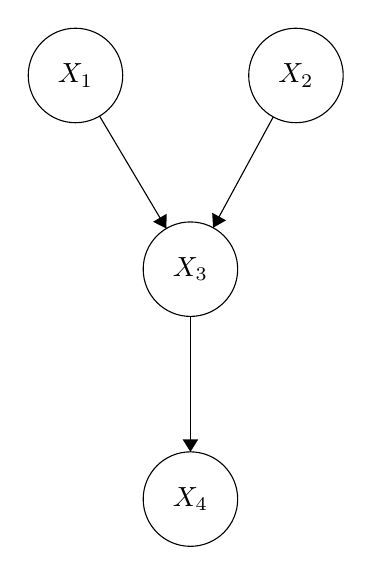
\begin{tikzpicture}[scale=0.2]
\tikzstyle{every node}+=[inner sep=0pt]
\draw [black] (38.4,-21.2) circle (3);
\draw (38.4,-21.2) node {$X_3$};
\draw [black] (31.1,-8.9) circle (3);
\draw (31.1,-8.9) node {$X_1$};
\draw [black] (45.1,-8.9) circle (3);
\draw (45.1,-8.9) node {$X_2$};
\draw [black] (38.4,-35.8) circle (3);
\draw (38.4,-35.8) node {$X_4$};
\draw [black] (32.63,-11.48) -- (36.87,-18.62);
\fill [black] (36.87,-18.62) -- (36.89,-17.68) -- (36.03,-18.19);
\draw [black] (43.66,-11.53) -- (39.84,-18.57);
\fill [black] (39.84,-18.57) -- (40.66,-18.1) -- (39.78,-17.62);
\draw [black] (38.4,-24.2) -- (38.4,-32.8);
\fill [black] (38.4,-32.8) -- (38.9,-32) -- (37.9,-32);
\end{tikzpicture}
\end{center}

We also have the associated conditional probability tables (as an example the top left element of table 3 reads as $P(X_3 = 0 | X_1 = 0, X_2 = 0) = 0.4$): \\

\begin{table}[H]
    \centering
    \begin{tabular}{|c|c|}
    \hline
         $X_1=0$ & $0.3$  \\ \hline
         $X_1=1$ & $0.7$    \\  \hline
    \end{tabular}
    \\ 
    \begin{tabular}{|c|c|}
    \hline
         $X_2=0$ & $0.5$  \\ \hline
         $X_2=1$ & $0.5$    \\  \hline
    \end{tabular}
    \\ 
    \begin{tabular}{|c|c|c|c|c|}
    \hline
            & $X_1=0, X_2=0$ & $X_1=0,X_2=1$ & $X_1=1,X_2=0$ & $X_1=1,X_2=1$   \\  \hline
        $X_3=0$ & $0.4$ & $0.7$ & $0.8$ & $0.5$ \\  \hline
        $X_3=1$ & $0.6$  & $0.3$ & $0.2$ & $0.5$    \\  \hline
    \end{tabular}
    \\
    \begin{tabular}{|c|c|c|}
    \hline
            & $X_3=0$ & $X_3=1$   \\  \hline
        $X_4=0$ & $0.8$ & $0.25$ \\  \hline
        $X_4=1$ & $0.2$  & $0.75$    \\  \hline
    \end{tabular}
    \\ 
    \caption{Conditional Probability tables}
\end{table}

In this section, we will test your understanding of several aspects of directed graphical models. For each question below, either write your answer as a fraction or write your answer to 5 decimal places (if needed).

\clearpage

\begin{questions}


\question[2]  What is $P(X_1=1, X_2=0, X_3=1, X_4=0)$?

\begin{your_solution}[title=Your Answer:,height=3cm,width=10cm]
\end{your_solution}

    
 
 
\question[2]  What is the value of $P(X_1=1)$?

\begin{your_solution}[title=Your Answer:,height=3cm,width=10cm]
\end{your_solution}

    
 
 
\question[2] What is the value of  $P(X_4=1)$?

\begin{your_solution}[title=Your Answer:,height=3cm,width=10cm]
\end{your_solution}

    
 
\question[2] What is $P(X_1 = 1, X_2=1, X_4=1)$?

\begin{your_solution}[title=Your Answer:,height=3cm,width=10cm]
\end{your_solution}

    
 
 \question[2] What is $P(X_2=1|X_4=1,X_3=0)$?

\begin{your_solution}[title=Your Answer:,height=3cm,width=10cm]
\end{your_solution}

    
 
 \clearpage
 
 \question[3] $(X_1 \independent X_2) | X_3$

\begin{checkboxes}
    \choice True
    \choice False
\end{checkboxes}


    
 
 \question[3] $(X_1 \independent X_4) | X_3$

\begin{checkboxes}
    \choice True
    \choice False
\end{checkboxes}


 
 \question[2]  What is the minimum number of parameters we must estimate in order to learn this graphical model?

\begin{your_solution}[title=Your Answer:,height=3cm,width=10cm]
\end{your_solution}

    
 
 \question[2]  If we made no assumptions about dependencies among random variables $X_1, X_2, X_3,$ and $X_4$ how many parameters would we need to estimate?

\begin{your_solution}[title=Your Answer:,height=3cm,width=10cm]
\end{your_solution}

 
 
 \question[2] Given random variables as $Z_1, Z_2, Z_3$, write a graphical model that reflects the following conditional independence assumption: $(Z_1 \independent Z_3)| Z_2$. You need only to draw the corresponding DAG of the model. You do not need to give the parameters of the model.
 
 \begin{your_solution}[title=Your Answer:,height=5cm,width=15cm]
\end{your_solution}

\clearpage
 
 \question[2] Given random variables as $Z_1, Z_2, Z_3$, write a graphical model that reflects NO conditional independencies among the variables. You may write the joint distribution of the model, or draw the corresponding DAG of the model.


 \begin{your_solution}[title=Your Answer:,height=5cm,width=15cm]
\end{your_solution}
 

\end{questions}


\clearpage


\section{Graphical Models: Learning Models}

\subsection{MLE and MAP}
Now consider the following graphical model:



\begin{center}
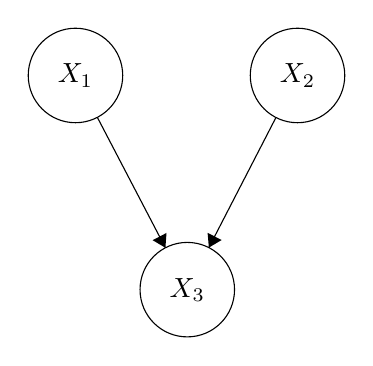
\begin{tikzpicture}[scale=0.2]
\tikzstyle{every node}+=[inner sep=0pt]
\draw [black] (37.9,-24) circle (3);
\draw (37.9,-24) node {$X_3$};
\draw [black] (30.8,-10.4) circle (3);
\draw (30.8,-10.4) node {$X_1$};
\draw [black] (44.9,-10.4) circle (3);
\draw (44.9,-10.4) node {$X_2$};
\draw [black] (43.53,-13.07) -- (39.27,-21.33);
\fill [black] (39.27,-21.33) -- (40.08,-20.85) -- (39.19,-20.39);
\draw [black] (32.19,-13.06) -- (36.51,-21.34);
\fill [black] (36.51,-21.34) -- (36.58,-20.4) -- (35.7,-20.86);
\end{tikzpicture}
\end{center}




We have the following observed data: \\
\begin{center}
\begin{tabular}{|c|c|c|}
    \hline
            $X_1$ & $X_2$ & $X_3$   \\  \hline
       $1$ & $0$ & $1$ \\  \hline
       $0$ & $0$ & $0$  \\  \hline
       $1$ & $1$ & $0$  \\  \hline
       $1$ & $1$ & $1$  \\  \hline
       $0$ & $1$ & $0$  \\  \hline
       $1$ & $0$ & $0$  \\  \hline
       $1$ & $0$ & $0$  \\  \hline
       $1$ & $1$ & $1$  \\  \hline
       $0$ & $0$ & $1$  \\  \hline
       $0$ & $0$ & $1$  \\  \hline
    \end{tabular}
\end{center}
    
    
\begin{questions}


\question[2] Given the data and the graphical model above, we would like to learn the parameters of the model using Maximum Likelihood Estimation. Write the Conditional Probability Distribution associated with $X_3$, use MLE estimates of the parameters based on this data. 

\begin{your_solution}[title=Your Answer:,height=5cm,width=15cm]
\end{your_solution}

\clearpage

\question[2] Now write a second set of parameter values, again for the Conditional Probability Distribution associated with $X_3$, but this time use MAP estimates with a Beta(2,2) prior.

\begin{your_solution}[title=Your Answer:,height=5cm,width=15cm]
\end{your_solution}

\end{questions}

\subsection{EM: Learning with Missing Data}
 Now suppose we have the same graphical model, but the data is sometimes missing the value of $X_3$. This gives the following data: \\
\begin{center}
\begin{tabular}{|c|c|c|}
    \hline
       $X_1$ & $X_2$ & $X_3$   \\  \hline
       $1$  & $0$ & $*$   \\  \hline
       $0$ & $0$ & $*$  \\  \hline
       $1$ & $1$ & $0$  \\  \hline
       $1$ & $1$ & $1$  \\  \hline
       $0$ & $1$ & $0$  \\  \hline
       $1$ & $0$ & $0$  \\  \hline
       $1$ & $0$ & $0$  \\  \hline
       $1$ & $1$ & $1$  \\  \hline
       $0$ & $0$ & $1$  \\  \hline
       $0$ & $0$ & $1$  \\  \hline
    \end{tabular}
\end{center}


There are now several parameters we cannot estimate directly since $X_3$ is missing: \\

$P(X_3=1|X_1=0,X_2=0)$ \\
$P(X_3=1|X_1=1,X_2=0)$ \\

To handle this missing data, we would like to use the EM algorithm as follows for boolean data: \\

\begin{enumerate}
    \item E-step: For each row (sample) $x_n$ that contains a missing value, use the observed features of row $\mathbf{x}_n$ and the current parameters $\theta$ to calculate $\mathbb{E}(\mathbf{z}_n|\mathbf{x}_n), \theta$, where $\mathbf{z}_n$ is the missing value(s) in that row.
    \item M-step: Re-estimate the parameters $\theta$ in a similar procedure to MLE on the fully observed data, but instead of counts of the unobserved variable use expected counts.
    \item Iterate until convergence, i.e. model likelihood has converged. 
\end{enumerate}

More explicitly in the boolean case for the model given, in the E-step for a given sample $n$ we calculate $\mathbb{E}(X_{n,3}) = \mathbb{E}(X_{n,3}|x_{n,1},x_{n,2},\theta)$, where $x_{n,i}$ denotes the $i$th variable in the $n$th sample.


Then, in the M-step, we re-estimate the parameters $\theta$ with the expected counts: $$\theta_{x_3|i,j} = \frac{\sum_{n=1}^{N} I(x_{n,1} = i, x_{n,2} = j)*\mathbb{E}(x_{n,3})}{\sum_{n=1}^{N} I(x_{n,1} = i, x_{n,2} = j)}$$ where $\theta_{x_3|i,j} = P(x_3 = 1| x_1 = i, x_2 = j)$.  Here $I(a)$ an "indicator" function, whose value is 1 if $a$ is true, and 0 otherwise.

\begin{questions}



\question[2] Execute the first E-step of the EM algorithm. More precisely, assume we initialize each unknown parameter to $0.5$, and other parameters to their MLE estimates. Give the expectations of the missing $X_3$ variables for row 1 and for row 2 in the data:

$\mathbb{E}(X_{1,3}|x_{1,1},x_{1,2},\theta)$: \\
\begin{your_solution}[title=Your Answer:,height=3cm,width=10cm]
\end{your_solution}


$\mathbb{E}(X_{2,3}|x_{2,1},x_{2,2},\theta)$: \\
\begin{your_solution}[title=Your Answer:,height=3cm,width=10cm]
\end{your_solution}

\clearpage

\question[6] Now execute the first M-step. List the estimated values of the unknown model parameters we obtain in this M-step. (Note that we use the expected count only when the variable is
unobserved in an example).

$\theta_{x_1}$: \\
\begin{your_solution}[title=Your Answer:,height=3cm,width=10cm]
\end{your_solution}


$\theta_{x_2}$: \\
\begin{your_solution}[title=Your Answer:,height=3cm,width=10cm]
\end{your_solution}

$\theta_{x_3 | 0,0}$: \\
\begin{your_solution}[title=Your Answer:,height=3cm,width=10cm]
\end{your_solution}


$\theta_{x_3 | 1,1}$: \\
\begin{your_solution}[title=Your Answer:,height=3cm,width=10cm]
\end{your_solution}

$\theta_{x_3 | 0,1}$: \\
\begin{your_solution}[title=Your Answer:,height=3cm,width=10cm]
\end{your_solution}
\clearpage

$\theta_{x_3 | 1,0}$: \\
\begin{your_solution}[title=Your Answer:,height=3cm,width=10cm]
\end{your_solution}



\question[2] Last, let’s simulate the second E-step. List the actual values for all the expectations
we calculate in this E-step. 

$\mathbb{E}(X_{1,3}|x_{1,1},x_{1,2},\theta)$: \\
\begin{your_solution}[title=Your Answer:,height=3cm,width=10cm]
\end{your_solution}


$\mathbb{E}(X_{2,3}|x_{2,1},x_{2,2},\theta)$: \\
\begin{your_solution}[title=Your Answer:,height=3cm,width=10cm]
\end{your_solution}



\end{questions}

\clearpage

\section{Programming Empirical Questions}

The following questions should be completed as you work through the programming component of this assignment.

\begin{questions}

\question[3] Using the data provided, plot the test accuracy (vertical axis) of the classifier versus the number of training examples used (horizontal axis) when using all 21,764 voxels. The data consists of 42 samples, and for each $i \in [10,...,42]$, plot the test accuracy of the classifier after training on the first $i$ samples in the train dataset.

\begin{your_solution}[title=Your Answer:,height=10cm,width=15cm]
\end{your_solution}

\clearpage

\question[3] Using the data provided, plot the test accuracy of your classifier (vertical axis) when training on all available training data, versus the top $k$ number of features you select (horizontal axis). Instead of plotting a point for each of the 21,764 values, plot a point for every 200 voxels starting at 50, so $k$ is in the set $[50,250,450,...,21650]$.

\begin{your_solution}[title=Your Answer:,height=10cm,width=15cm]
\end{your_solution}

\clearpage

\question[2] Using the visualization tool, submit two slices of your choice, one for the building class and one for the tool class, that show a visual difference in the neural activation patterns. Comment briefly on your observations. See \ref{visualize} for details on generating the output. 

\begin{your_solution}[title=Your Answer:,height=18cm,width=15cm]
\end{your_solution}

\end{questions}
\newpage
\end{questions}

{\LARGE \bf Programming (40 points)}


\section{The Task}
In this task, you will be using Gaussian Naive Bayes to predict the word stimulus given to a human subject based on their observed neural activity measured by functional magnetic resonance imaging (fMRI). 

Studies have shown that thinking about different semantic categories of words (for example, tools, buildings, and animals) activates different spatial patterns of neural activation in the brain. A study conducted in 2008 generated a computational model which predicts the fMRI neural activation associated with thinking about arbitrary concrete nouns.  

In this homework you will use the data from that study for a different purpose: to train a Naive Bayes classifier to predict which category of words (e.g., tools, buildings, vehicles) the person is reading, based on their fMRI neural image. For this assignment you will only be distinguishing between two categories: tools and buildings. 


The programs you write will be automatically graded using the Gradescope system. You may write your programs in \textbf{Python, Java, or C++}. However, you should use the same language for all parts below.
\linebreak

\section{The Datasets}
\label{sec:dataset}

\paragraph{Datasets} 
The fMRI dataset used in this experiment was originally collected by Marcel Just and his colleagues in Carnegie Mellon University's CCBI. Seventeen 5-mm thick oblique-axial slices were imaged with a gap of 1-mm between slices, normalized, and resampled to 3x3x6 mm3 voxels. Thus, each fMRI image in the dataset is represented as 21,764 voxels (3D pixels).


\paragraph{File Format} The dataset consists of two files: train\_data.csv and test\_data.csv. Each row in the file represents one example: a brain image, and the label to be predicted (the category of the word the person was reading when this brain image was collected). Each row contains 21,765 columns separated by commas. Columns 1 through 21,764 represent the voxels making up the fMRI image. The last column in each row contains the label, which can be one of two categories: ``tool" or ``building". 

 \vspace{5mm}
\section{Model Definition}
\label{Model Definition}

To predict the word stimulus category given the fMRI voxels, you will use a Gaussain Naive Bayes model. Whereas in class we discussed Bernoulli Naive Bayes when the input features were binary, here we are using Gaussian Naive Bayes since the voxel values for each feature are continuous. \\

Formally, if we have input features $\mathbf{x} \in \mathbb{R}^M$ and labels $y \in \{0,1\}$, the ``Gaussian" aspect of Gaussian Naive Bayes assumes that $$P(x_m |y=k) \sim \mathcal{N}(\mu_{m,k}, \sigma_{m,k}) \quad \forall m \in [1,...,M], k \in \{0,1\}$$ i.e. the probability of a feature $m$ given the class $k$ comes from a normal distribution with parameters $\mu_{m,k}, \sigma_{m,k}$.

So, we have $$P(X_m = v | y = k) = \frac{1}{\sqrt{2\pi\sigma_{m,k}^2}} \exp{(\frac{-(v-\mu_{m,k})^2}{2\sigma_{m,k}^2})}$$ which is the Gaussian PDF parameterized by $\mu_{m,k}$ and $\sigma_{m,k}$.

Under this Gaussian assumption along with the Naive Bayes assumption, we have the following generative model for the data with binary labels and continuous features: 

$$p(\mathbf{x},y) = p(y)\prod_{m=1}^{M} p(x_m|y)$$ where $p(x_m|y)$ is a normal distribution as defined above. \\

Classification:

After learning a generative model, we would like to be able to perform classification for our binary labelling task. In order to do so for input $\mathbf{x}$ we compute our prediction $$\hat{y} = \argmax_y p(y|\mathbf{x})$$. \\



%Support: Continuous vectors $\mathbf{x} \in \mathbb{R}^M$ \\

%Generative Story: 
%\begin{itemize}
%    \item $Y \sim \text{Bernoulli}(\phi)$
%    \item $X_m \sim \mathcal{N}(\mu_{m,Y},\sigma_{m,Y}) \quad %\forall m \in [1,...,M]$
%\end{itemize}

\section{MLE Estimation}

To learn the model, we would first like to use MLE to estimate the model parameters. Assume we have a dataset $\mathcal{D} = \{(\mathbf{x}^{(i)},y^{(i)})\}_{i=1}^N$

To estimate $P(Y=1)$ using MLE, since $Y$ is a binary value we end up with $$P(Y=1) = \frac{\#D\{Y=1\}}{|D|}$$ where $\#D\{Y=1\}$ is the count of items in dataset $D$ where $Y = 1$. 

We also need to estimate $P(X_m = v| Y = k)$ for each feature $i$. To do so, for a given class and since each feature is continuous, we need to estimate a class-conditional Gaussian distribution with parameters $\mu$ and $\sigma$ as explained in \ref{Model Definition}


Thus, for feature $m$ and class $k$ and, we estimate $\hat{\mu}_{m,k}$ as $$\frac{1}{\sum_{i=1}^{N} I(Y^{(i)} = k)} \sum_{i=1}^{N} \mathbf{x}^{(i)}_m * I (Y^{(i)} = k)$$

We also estimate $\hat{\sigma}_{m,k}^2$ as $$\frac{1}{\sum_{i=1}^{N} I(Y^{(i)} = k)} \sum_{i=1}^{N} (\mathbf{x}^{(i)}_m - \hat{\mu}_{m,k})^2*I (Y^{(i)} = k)$$

\section{Log-Space Arithmetic}

In computing $P(Y|X)$ via Bayes' Rule, we end up with $$P(Y|X) = \frac{P(X|Y)P(Y)}{P(X)} \propto P(X|Y)P(Y)$$. If $X$ is a vector of size $M$ where $M$ is very large, we end up with a large product of probabilities: $$\prod_{i=1}^{M} P(X_i|Y) P(Y)$$.

To avoid underflow problems (reaching an incorrect value of 0 when multiplying many probabilities that are $\leq 1$), we can convert the computation to log-space. 

As a result, instead of computing $P(Y|X)$, you should compute $$\log(P(Y|X)) = \log(P(Y)) + \sum_{i=1}^{M} \log(P(X_i|Y))$$ where we use the natural logarithm base. 

\section{Feature Selection}
\label{features}

After building the Gaussian Naive Bayes classifier, we would like to optimize our performance by extracting only the top $k$ useful features.

This can be done by selecting features whose mean given the label is `tool' is very different from the mean given the label is `building'. For example, the `best' feature would maximize

       $$ \lvert \mu_{m,tool} - \mu_{m,building} \rvert $$
       
       
\section{Implementation}
Write a program \texttt{gnb.\{py|java|cpp|m\}} that implements a binary classifier using Gaussian Naive Bayes. Your program should output the predictions and error rates on the train and test datasets with training done on the top $k$ voxels, where $k$ is specified from the command line parameter \textit{num\_voxels}. 


\textbf{Note}:
Because computing the joint probability involves repeated multiplications, you will need to work in \emph{log space} to prevent underflow. 


\subsection{Command Line Arguments}
\label{sec:args}
The autograder runs and evaluates the output from the files generated, using the following command:

\begin{tabular}{ll}
For Python: &
\begin{lstlisting}[language=Shell]
$ python3 gnb.py [args...]
\end{lstlisting}
\\
For Java: &
\begin{lstlisting}[language=Shell]
$ javac -cp "./lib/ejml-v0.38-libs/*:./" gnb.java
$ java -cp "./lib/ejml-v0.38-libs/*:./" gnb [args...]
\end{lstlisting}
\\
For C++: &
\begin{lstlisting}[language=Shell]
$ g++ -g -std=c++11 -I./lib gnb.cpp; ./a.out [args...]
\end{lstlisting}
\end{tabular}

Where above \texttt{[args\dots]} is a placeholder for six command-line arguments. These arguments are described in detail below:
\begin{enumerate}
    \item \texttt{<train\_input>}: path to the training input \texttt{.csv} file (see Section~\ref{sec:dataset})
    \item \texttt{<test\_input>}: path to the test \ input \texttt{.csv} file (see Section~\ref{sec:dataset})
    \item \texttt{<train\_out>}: path to output \texttt{.labels} file to which the prediction on the \emph{train} data should be written (see Section~\ref{output})
    \item \texttt{<test\_out>}: path to output \texttt{.labels} file to which the prediction on the \emph{test} data should be written (see Section~\ref{output})
     \item \texttt{<metrics\_out>}: path of the output \texttt{.txt} file to which metrics such as train and validation\thinspace error should be written  (see Section~\ref{metrics})
    \item \texttt{<num\_voxels>}: an integer denoting that the top \texttt{num\_voxels} found via the feature selection method described should be used for training the gnb classifer (see Section~\ref{features})

\end{enumerate}

As an example, if you implemented your program in Python, the following command line would run your program.
\\
\begin{lstlisting}[language=Shell]
$ python3 gnb.py train_data.csv test_data.csv train_out.labels 
\ test_out.labels metrics_out.txt 21764

\end{lstlisting}

\subsection{Output: Labels Files} \label{output}
Your program should output a \texttt{.labels} file containing the predictions of your model on training data (\texttt{<train\_out>}) and test\thinspace data (\texttt{<test\_out>}) with training done on the top \textit{num\_voxels} voxels as specified from the command line input. The file should contain the predicted labels for each example printed on a new line. Use \lstinline{\n} to create a new line. 

Your labels should exactly match those of a reference implementation -- this will be checked by the autograder by running your program and evaluating your output file against the reference solution.

\textbf{Note}: You should output your predicted labels using the same \emph{string} identifiers as the original training data: either 'tool' or 'building'. 

A few lines of sample output is given below. 

\begin{lstlisting}
building
building
tool
\end{lstlisting}

\subsection{Output Metrics} \label{metrics}
Generate the train and test errors from your Gaussian Naive Bayes classifier. You must output a metric file containing the train and test errors as shown below. 

%All of your reported numbers should be within 0.01 of the reference solution. 
A sample output is given below. 

\begin{lstlisting}
error(train): 0.000000
error(test): 0.000000
\end{lstlisting}

Take care that your output has the exact same format as shown above. Each line should be terminated by a Unix line ending \lstinline{\n}.


\section{Visualization}
\label{visualize}
We have provided for you a visualization tool for you to view horizontal slices of the brain from the fMRI scans.

The script takes in two arguments: 1) the path to the dataset of your choice, and 2) a row index into the dataset corresponding to the image you would like to visualize. 

Here is an example of how to run the tool: 
\\
\begin{lstlisting}[language=Shell]
$ python3 visualize.py <path_to_dataset> <row_index>
\end{lstlisting}


Below is an example of what an output slice should look like. Note the back of the head corresponds to $x=0$ in this plot, and the front of the head to $x=59$. The bright yellow (high positive activation) region around ($x=11, y=25)$ is part of visual cortex. Dark blue regions indicate lower than average activation.  The empty regions inside the brain are the white matter of the brain (the axons, but not the firing cortical regions, so we mask out fMRI activity in these regions).


\begin{center}
\includegraphics[width=300px]{images/visualization.png}
\end{center}

\section{Gradescope Submission}
You should submit your \texttt{gnb.\{py|java|cpp\}} and a to Gradescope. Please do not use any other file name for your implementation. This will cause problems for the autograder to correctly detect and run your code.
\newpage

\end{document}